\section{Introduction}

Let $H_0 \colon \C \to \C$ denote the function
\begin{equation}\label{hoz}
 H_0(z) \coloneqq \frac{1}{8} \xi\left(\frac{1}{2} + \frac{iz}{2}\right),
\end{equation}
where $\xi$ denotes the Riemann $\xi$ function
\begin{equation}\label{sas}
 \xi(s) \coloneqq \frac{s(s-1)}{2} \pi^{-s/2} \Gamma\left(\frac{s}{2}\right) \zeta(s)
\end{equation}
(after removing all singularities) and $\zeta$ is the Riemann $\zeta$ function.
Then $H_0$ is an entire even function with functional equation $H_0(\overline{z}) = \overline{H_0(z)}$, and the Riemann hypothesis (RH) is equivalent to the assertion that all the zeroes of $H_0$ are real.

It is a classical fact (see \cite[p. 255]{titch}) that $H_0$ has the Fourier representation
$$ H_0(z) = \int_0^\infty \Phi(u) \cos(zu)\ du$$
where $\Phi$ is the super-exponentially decaying function
\begin{equation}\label{phidef}
 \Phi(u) \coloneqq \sum_{n=1}^\infty (2\pi^2  n^4 e^{9u} - 3\pi n^2 e^{5u} ) \exp(-\pi n^2 e^{4u} ).
\end{equation}
The sum defining $\Phi(u)$ converges absolutely for negative $u$ also.  From Poisson summation one can verify that $\Phi$ satisfies the functional equation $\Phi(u) = \Phi(-u)$ (i.e., $\Phi$ is even); this fact is of course closely related to the functional equation for $\zeta$. 

De Bruijn \cite{debr} introduced (with somewhat different notation) the more general family of functions $H_t \colon \C \to \C$ for $t \in \R$, defined by the formula
\begin{equation}\label{htdef}
 H_t(z) \coloneqq \int_0^\infty e^{tu^2} \Phi(u) \cos(zu)\ du.
\end{equation}
As noted in \cite[p.114]{csv}, one can view $H_t$ as the evolution of $H_0$ under the backwards heat equation $\partial_t H_t(z)= -\partial_{zz} H_t(z)$.
As with $H_0$, each of the $H_t$ are entire even functions with functional equation $H_t(\overline{z}) = \overline{H_t(z)}$; from the super-exponential decay of $e^{tu^2} \Phi(u)$ we see that the $H_t$ are in fact entire of order $1$.  It follows from the work of P\'olya \cite{polya} that if $H_t$ has purely real zeroes for some $t$, then $H_{t'}$ has purely real zeroes for all $t'>t$; de Bruijn showed that the zeroes of $H_t$ are purely real for $t \geq 1/2$.  Newman \cite{newman} strengthened this result by showing that there is an absolute constant $-\infty < \Lambda \leq 1/2$, now known as the \emph{De Bruijn-Newman constant}, with the property that $H_t$ has purely real zeroes if and only if $t \geq \Lambda$.  The Riemann hypothesis is then clearly equivalent to the upper bound $\Lambda \leq 0$.  Recently in \cite{brad} the complementary bound $\Lambda \geq 0$ was established, answering a conjecture of Newman \cite{newman}, and improving upon several previous lower bounds for $\Lambda$ \cite{cnv,nrv,crv,cosv,odlyzko,saouter}.  Furthermore, Ki, Kim, and Lee \cite{kkl} sharpened the upper bound $\Lambda \leq 1/2$ of de Bruijn \cite{debr} slightly to $\Lambda < 1/2$.  

In this paper we improve the upper bound:

\begin{theorem}[New upper bound]\label{new-upper}  We have $\Lambda \leq 0.22$.
\end{theorem}

The proof of Theorem \ref{new-upper} combines numerical verification with some new asymptotics and observations about the $H_t$ which may be of independent interest.  Firstly, by analyzing the dynamics of the zeroes of $H_t$, we establish in Section \ref{dynamics-sec} the following criterion for obtaining upper bounds on $\Lambda$:

\begin{theorem}[Upper bound criterion]\label{ubc-0}  Suppose that $t_0, X > 0$ and $0 < y_0 \leq 1$ obey the following hypotheses:
\begin{itemize}
\item[(i)]  (Numerical verification of RH at initial time $0$) There are no zeroes $\zeta(\sigma+iT) = 0$ with $\frac{1+y_0}{2} \leq \sigma \leq 1$ and $0 \leq T \leq \frac{X}{2}$.
\item[(ii)]  (Asymptotic zero-free region at final time $t_0$) There are no zeroes $H_{t_0}(x+iy)=0$ with $x \geq X+\sqrt{1-y_0^2}$ and $y_0 \leq y \leq \sqrt{1-2t_0}$.
\item[(iii)]  (Barrier at intermediate times) There are no zeroes $H_{t}(x+iy)=0$ with $X \leq x \leq X+\sqrt{1-y_0^2}$, $\sqrt{y_0^2+2(t_0-t)} \leq y \leq \sqrt{1-2t}$, and $0 \leq t \leq t_0$.
\end{itemize}
Then $\Lambda \leq t_0 + \frac{1}{2} y_0^2$.
\end{theorem}

Informally, hypothesis (i) implies that at time $t=0$, there are no zeroes $H_t(x+iy)=0$ with large values of $y$ to the left of the barrier region in (iii).  The absence of zeroes in that barrier, together with a continuity argument and an analysis of the time derivative of each zero, can then be used to show that for later times $0 < t \leq t_0$, there continue to be no zeroes $H_t(x+iy)=0$ with large values of $y$ to the left of the barrier; see Figure \ref{barrier-fig}.  Hypothesis (ii) then gives the complementary assertion to the right of the barrier, and one can use an existing theorem of de Bruijn (Theorem \ref{debr-bound}) to conclude.

In practice, we have found it convenient numerically to replace the barrier region in Theorem \ref{ubc-0} with the larger and simpler region
$$ X \leq x \leq X+1; \quad y_0 \leq y \leq 1; \quad 0 \leq t \leq t_0.$$

\begin{figure}[ht!]
  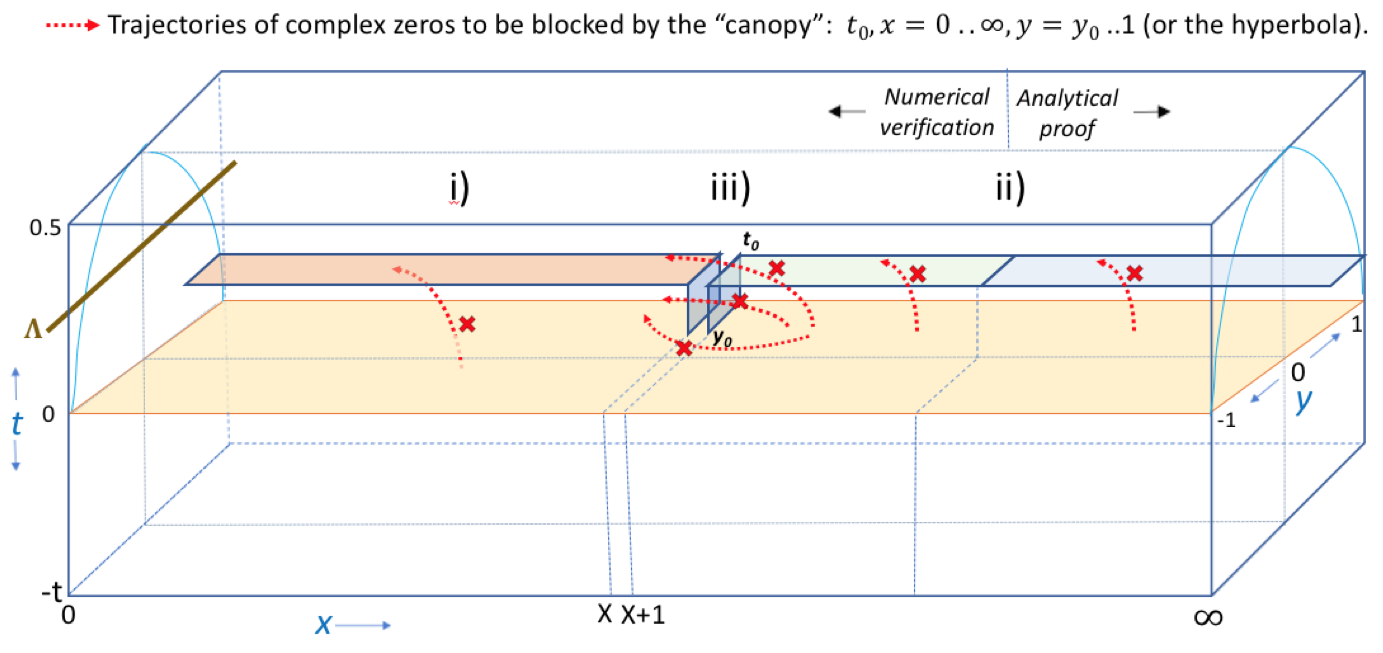
\includegraphics[width=0.9\linewidth]{Barrier_approach.png}
  \caption{A visualization of Theorem \ref{ubc-0}.  If at time $t_0$ one can show that there are no zeroes $H_t(x+iy)=0$ in the ``canopy'' $0 \leq x <\infty$, $y_0 \leq y \leq 1$, then a theorem of de Bruijn allows one to conclude the desired bound $\Lambda \leq t_0 + \frac{1}{2} y_0^2$.  The hypothesis (i) prevents zeroes hitting this canopy from an initial position to the left of the barrier; the hypothesis (ii) prevents zeroes from lying in the canopy to the right of the barrier; and the hypothesis (iii) prevents zeroes from starting to the right of the barrier and reaching the canopy to the left of the barrier.}
\label{barrier-fig}
\end{figure}

We will obtain Theorem \ref{new-upper} by applying Theorem \ref{ubc-0} with the specific numerical choices $t_0 = 0.2$, $X = 6 \times 10^{10} + 83952 - 0.5$, and $y_0 = 0.2$.  The reason we choose $X$ close to $6 \times 10^{10}$ is that this is near the limit of known numerical verifications of the Riemann hypothesis such as \cite{platt}, which we need for the hypothesis (i) of the above theorem; the shift $83952 - 0.5$ is in place to make the partial Euler product $\prod_{p \leq 11} \left(1 - \frac{1}{p^{\frac{1-iX}{2}}}\right)^{-1}$ large, which helps in keeping the functions $H_t(x+iy), H_{t_0}(x+iy)$ large in magnitude, which in turn is helpful for numerical verifications of (ii) and (iii); see also Figure \ref{euler}.  The choices $t_0=0.2, y_0=0.2$ are then close to the limit of our ability to numerically verify hypothesis (ii) for this choice of $X$.  (The hypothesis (iii) is also verified numerically, but can be done quite quickly compared to (ii), and so does not present the main bottleneck to further improvements to Theorem \ref{new-upper}.)  Further upper bounds to $\Lambda$ can be obtained if one assumes the Riemann hypothesis to hold up to larger heights than that in \cite{platt}: see Section \ref{further-sec}.

To verify (ii) and (iii), we need efficient approximations (of Riemann-Siegel type) for $H_t(x+iy)$ in the regime where $t,y$ are bounded and $x$ is large.  For sake of numerically explicit constants, we will focus attention on the region
\begin{equation}\label{region}
0 < t \leq \frac{1}{2}; \quad 0 \leq y \leq 1; \quad x \geq 200,
\end{equation}
though the results here would also hold (with different explicit constants) if the numerical quantities $\frac{1}{2}, 1, 200$ were replaced by other quantities.

A key difficulty here is that $H_t(x+iy)$ decays exponentially fast in $x$ (basically because of the Gamma factor in \eqref{sas}); see Figure \ref{loghtandlogbt}.  This means that any direct attempt to numerically establish a zero-free region for $H_t(x+iy)$ for large $x$ would require enormous amounts of numerical precision.  To get around this, we will first renormalise the function $H_t(x+iy)$ by dividing it by a nowhere vanishing explicit function $B_t(x+iy)$ (basically a variant of the aforementioned Gamma factor) that removes this decay.  To describe this function, we first introduce the function $M_0: \C \backslash (-\infty,1] \to \C \backslash \{0\}$ defined by the formula
\begin{equation}\label{M-def}
 M_0(s) \coloneqq \frac{1}{8} \frac{s(s-1)}{2} \pi^{-s/2} \sqrt{2\pi} \exp\left( \left(\frac{s}{2}-\frac{1}{2}\right)\Log \frac{s}{2} - \frac{s}{2} \right),
\end{equation}
where $\Log$ denotes the standard branch of the complex logarithm, with branch cut at the negative axis and imaginary part in $(-\pi,\pi]$. One may interpret $M_0(s)$ as the Stirling approximation to the factor $\frac{1}{8} \frac{s(s-1)}{2} \pi^{-s/2} \Gamma\left(\frac{s}{2}\right)$ appearing in \eqref{hoz}, \eqref{sas}; it decays exponentially as one moves to infinity $s \to \pm i \infty$ along the critical strip.  We may form a holomorphic branch $\log M_0: \C \backslash (-\infty,1] \to \C$ of the logarithm of $M_0$ by the formula
\begin{equation}\label{logM}
 \log M_0(s) \coloneqq \Log s + \Log(s-1) - \frac{s}{2} \log \pi + \log \frac{\sqrt{2\pi}}{16} + 
 \left(\frac{s}{2}-\frac{1}{2}\right)\Log \frac{s}{2} - \frac{s}{2};
\end{equation}
differentiating this, we see that the logarithmic derivative $\alpha: \C \backslash (-\infty,1] \to \C$ of this function, defined by
\begin{equation}\label{alpha-def}
\alpha \coloneqq (\log M_0)' = \frac{M'_0}{M_0}
\end{equation}
is given explicitly by the formula
\begin{equation}\label{alpha-form}
\begin{split}
 \alpha(s) &= \frac{1}{s} + \frac{1}{s-1} - \frac{1}{2} \log \pi + \frac{1}{2} \Log \frac{s}{2} - \frac{1}{2s} \\
&= \frac{1}{2s} + \frac{1}{s-1} + \frac{1}{2} \Log \frac{s}{2\pi}.
\end{split}
\end{equation}
For any time $t \in \R$, we then define the deformation $M_t: \C \backslash (-\infty,1]$ of $M_0$ by the formula
\begin{equation}\label{Mt-def}
M_t(s) \coloneqq \exp\left( \frac{t}{4} \alpha(s)^2 \right) M_0(s)
\end{equation}
for any $t \geq 0$.
In the region \eqref{region}, we introduce the quantity
\begin{equation}\label{bo-def} 
B_t(x+iy) \coloneqq M_t\left(\frac{1+y-ix}{2}\right).
\end{equation} 
For fixed $t \geq 0$ and $y>0$, $B_t(x+iy)$ is non-vanishing, and it is easy to verify the asymptotic $|B_t(x+iy)| = e^{-(\frac{\pi}{8} + o(1)) x}$.  As it turns out, $B_t(x+iy)$ is an asymptotic approximation to $H_t(x+iy)$ in the region \eqref{region}, in the sense that
\begin{equation}\label{limx}
 \lim_{x \to \infty} \frac{H_t(x+iy)}{B_t(x+iy)} = 1
\end{equation}
for any fixed $t>0$ and $y>0$; see Figure \ref{ht-bt}.  (However, the convergence of \eqref{limx} is \emph{not} uniform as $t$ approaches zero.)

\begin{figure}[ht!]
  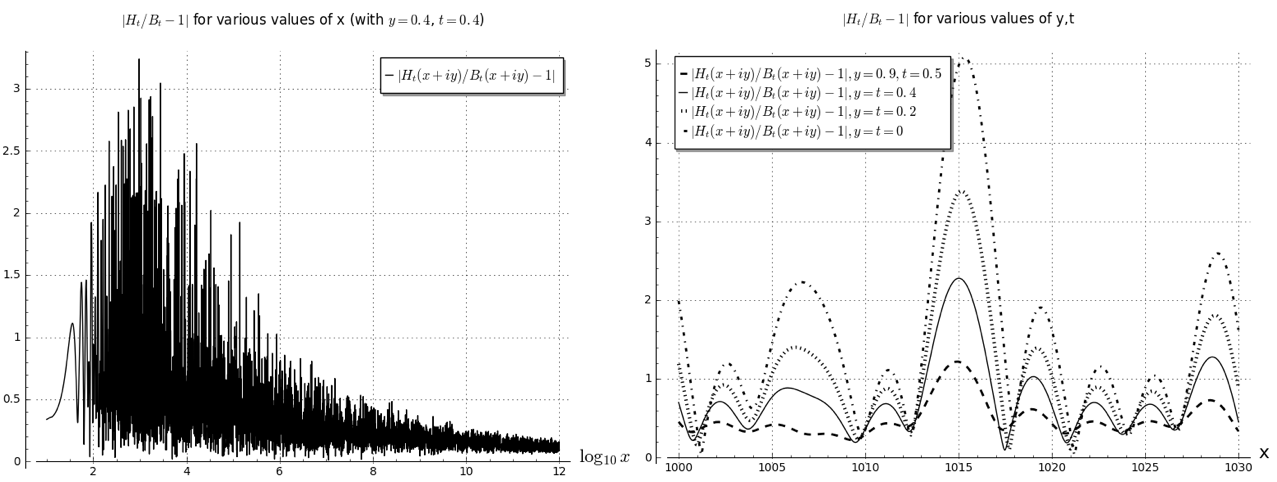
\includegraphics[width=1.0\linewidth]{ftvsht.png}
  \caption{The quantity $|H_t(x+iy)/B_t(x+iy) - 1|$ when $y=t=0.4$ and $\log_{10} x \leq 12$ (left) and when for $1000 \leq x \leq 1030$ and various choices of $(y,t)$ (right).}
\label{ht-bt}
\end{figure}

\begin{figure}[ht!]
  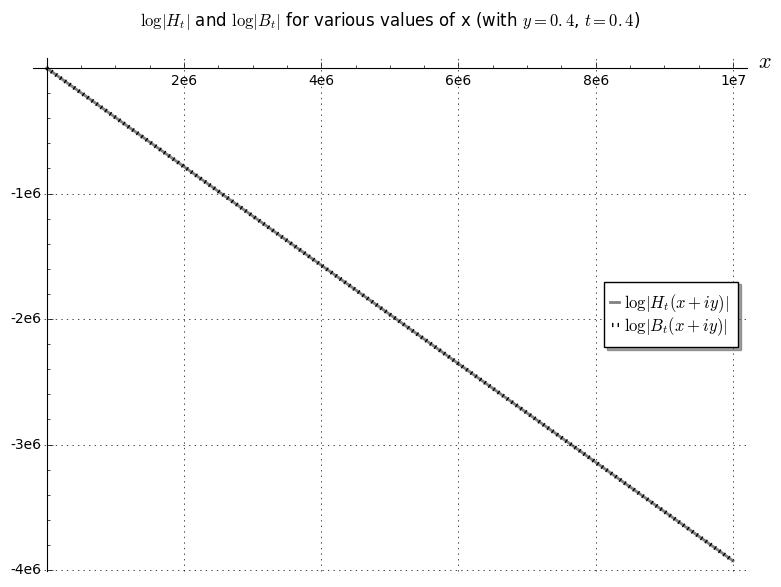
\includegraphics[width=0.8\linewidth]{loghtbt.png}
  \caption{The quantities $\log|H_t(x+iy)|$ and $\log|B_t(x+iy)|$ when $y=t=0.4$ and $\log_{10} x \leq 7$.   Both quantities decay like $- \frac{\pi}{8} x \approx -0.393 x$.}
\label{loghtandlogbt}
\end{figure}

In fact we have the following significantly more accurate approximation (of Riemann-Siegel type) with effective error estimates.
For any real number $X$, let $O_{\leq}(X)$ denote a quantity that is bounded in magnitude by $X$. We also use $x_+ = \max(x,0)$ to denote the positive part of a real number $x$.

\begin{theorem}[Effective Riemann-Siegel approximation to $H_t(x+iy)$]\label{eff}  Let $t,x,y$ lie in the region \eqref{region}.  Then we have
\begin{equation}\label{ratio-form-eff}
\frac{H_t(x+iy)}{B_t(x+iy)} = f_t(x+iy) + O_{\leq}\left( e_A + e_B + e_{C,0} \right)
\end{equation}
where
\begin{align}
f_t(x+iy) &\coloneqq \sum_{n=1}^N \frac{b_n^t}{n^{s_*}} + \gamma \sum_{n=1}^N n^y \frac{b_n^t}{n^{\overline{s_*} + \kappa}}\label{ft-def} \\
b_n^t &\coloneqq \exp( \frac{t}{4} \log^2 n ) \label{bn-def}\\
\gamma = \gamma(x+iy) &\coloneqq \frac{M_t\left(\frac{1-y+ix}{2}\right)}{M_t\left(\frac{1+y-ix}{2}\right)} \label{lambda-def} \\
s_* = s_*(x+iy) &\coloneqq \frac{1+y-ix}{2} +\frac{t}{2} \alpha\left(\frac{1+y-ix}{2}\right) \label{sn-def}\\
\kappa = \kappa(x+iy) &\coloneqq \frac{t}{2} \left(\alpha\left(\frac{1-y+ix}{2}\right) - \alpha\left(\frac{1+y+ix}{2}\right)\right) \label{kappa-def}\\
N &\coloneqq \left\lfloor \sqrt{\frac{x}{4\pi} + \frac{t}{16}} \right\rfloor \label{N-def-main} 
\end{align}
and $e_A, e_B, e_{C,0}$ are certain explicitly computable positive quantities\footnote{See \eqref{ea-def}-\eqref{ec-def} for the precise definition of these quantities.} depending on $t$ and $x+iy$.  Furthermore, we have the following bounds:
\begin{align}
|\gamma| &\leq e^{0.02 y} \left( \frac{x}{4\pi} \right)^{-y/2}  \label{gamma-bound} \\
\mathrm{Re} s_* &\geq \frac{1+y}{2} +\frac{t}{4} \log \frac{x}{4\pi} - \frac{t}{2x^2} \left(1-3y+\frac{4y(1+y)}{x^2}\right)_+  \label{res-bound} \\
|\kappa| &\leq  \frac{ty}{2(x-6)} \label{kappa-bound} \\
e_A + e_B &\leq \sum_{n=1}^N (1 + |\gamma| N^{|\kappa|} n^y) \frac{b_n^t}{n^{\mathrm{Re}(s_*)}} \left( \exp\left( \frac{\frac{t^2}{16} \log^2 \frac{x}{4\pi n^2} + 0.626}{x-6.66} \right)-1 \right) \label{eab-bound} \\
e_{C,0} &\leq \left(\frac{x}{4\pi}\right)^{-\frac{1+y}{4}} \exp\left( - \frac{t}{16} \log^2 \frac{x}{4\pi} + \frac{1.24 \times (3^y+3^{-y})}{N-0.125} + \frac{3 |\log \frac{x}{4\pi} + i \frac{\pi}{2}|+10.44}{x-8.52} \right) \label{ec-bound}
\end{align}
\end{theorem}

This theorem will be proven in Section \ref{initial-sec}; see Figures \ref{htft}, \ref{htft-2} for a numerical illustration of the approximation.  The strategy is to express $H_t$ as a convolution of $H_0$ with a gaussian heat kernel, then apply an effective Riemann-Siegel expansion to $H_0$ to rewrite $H_t$ as the sum of various contour integrals; see Section \ref{heatflow-sec} for details.  One then uses the saddle point method to shift each such contour to a location that is suitable for effective estimation.   We remark that $f_t(x+iy)$ is a holomorphic function of $x+iy$ in the region \eqref{region} as long as $N$ is constant, but has jump discontinuities when $N$ is incremented.

\begin{figure}[ht!]
  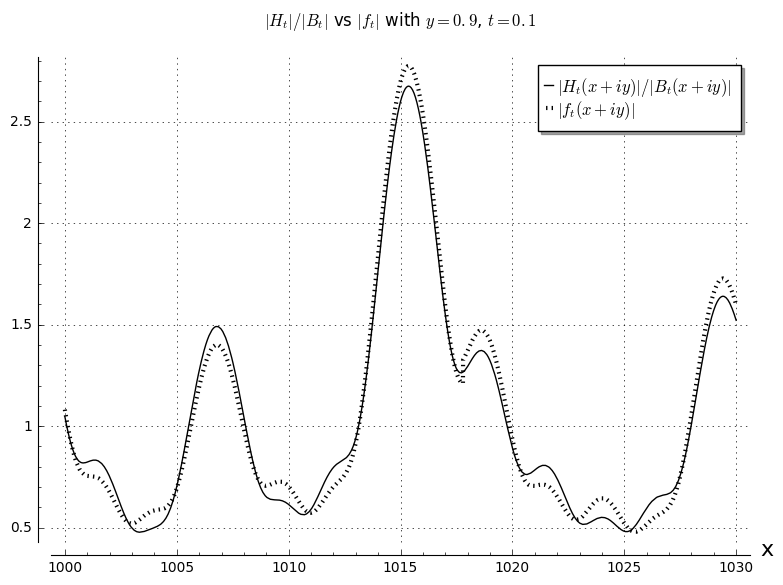
\includegraphics[width=\linewidth]{ft_vs_HtdivBt_y_09.png}
  \caption{Comparison of $|f_t(x+iy)|$ and $|H_t(x+iy)|/|B_t(x+iy)|$ for $y=0.9$, $t=0.1$, $1000 \leq x \leq 1030$, (left) and when $10^6 \leq x \leq 10^6 + 30$ (right). The approximation improves as $x$ gets larger.}
	\label{htft}
\end{figure}

\begin{figure}[ht!]
  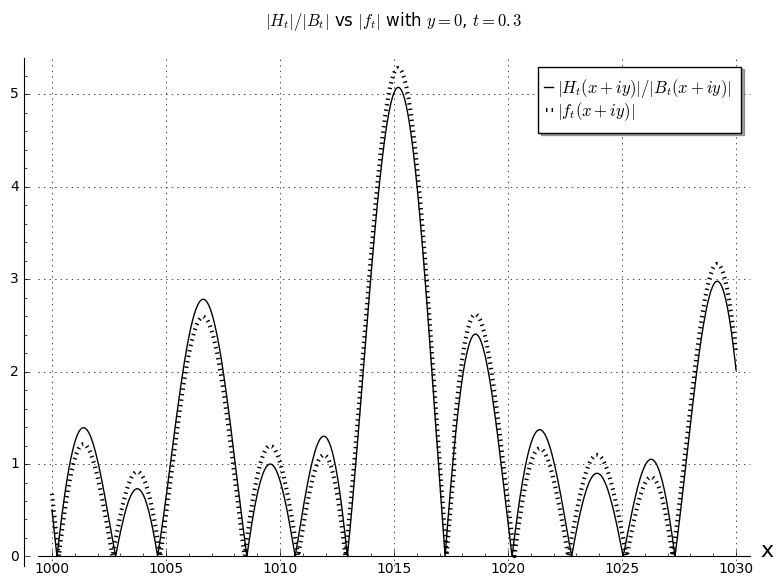
\includegraphics[width=\linewidth]{ft_vs_HtdivBt_y_0.png}
  \caption{Comparison of $|f_t(x+iy)|$ and $|H_t(x+iy)|/|B_t(x+iy)|$ for $y=0$, $t=0.3$, $1000 \leq x \leq 1030$ (left), and when $10^6 \leq x \leq 10^6 + 30$ (right). Again notice the improving approximation with $x$.}
	\label{htft-2}
\end{figure}

\begin{figure}[ht!]
  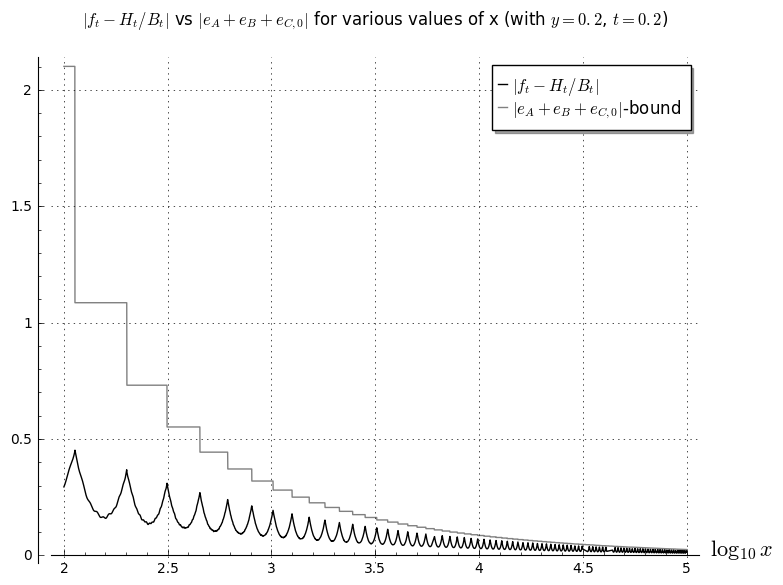
\includegraphics[width=0.8\linewidth]{ft_min_Ht_vs_errorterms.png}
  \caption{The error upper bound $|e_A+e_B+e_{C,0}|$ versus $|f_t - H_t/B_t|$ when $y=t=0.2$ and $2 \leq \log_{10} x \leq 5$.}
\label{errorboundtot}
\end{figure}

\begin{figure}[ht!]
  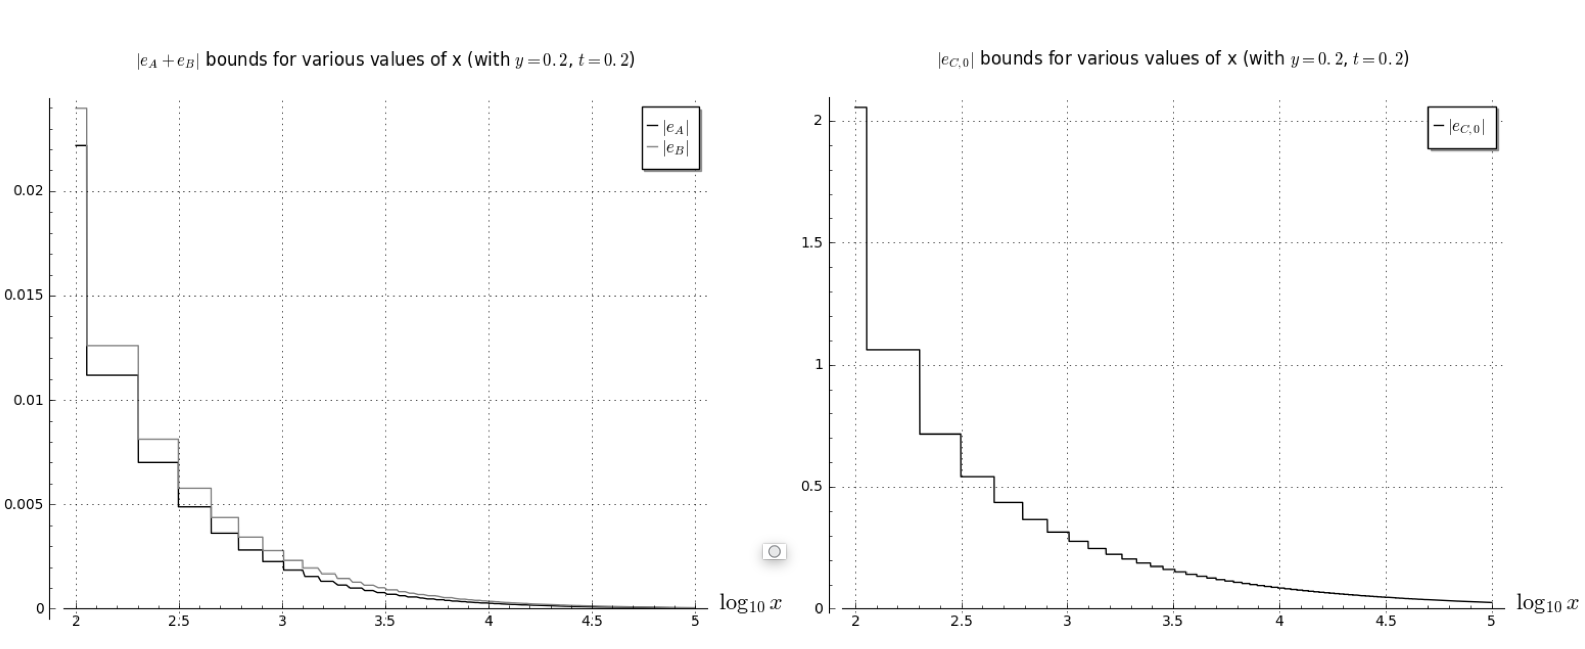
\includegraphics[width=1.0\linewidth]{eA_eB_eC_errorbounds.png}
  \caption{The individual error upper bounds $|e_A|$, $|e_B|$ and $|e_{C,0}|$ with $y=t=0.2$ and $2 \leq \log_{10} x \leq 5$. The $e_{C,0}$-term clearly dominates.}
\label{ind_errorbounds}
\end{figure}

From \eqref{ratio-form-eff} and the triangle inequality, we have a numerically verifiable criterion to establish non-vanishing of $H_t$ at a given point:

\begin{corollary}[Criterion for non-vanishing]\label{zero-test}  Let $t,x,y$ lie in the region \eqref{region}, and let $f_t, e_A, e_B, e_{C,0}$ be as in Theorem \ref{eff}.  If one has the inequality
\begin{equation}\label{criterion}
|f_t(x+iy)| > e_A + e_B + e_{C,0} 
\end{equation}
then $H_t(x+iy) \neq 0$.  
\end{corollary}

Actually, for some regions of $x,y,t$ we will use a more complicated criterion than \eqref{criterion}, in order to exploit the argument principle.  To numerically estimate $f_t(x+iy)$ in a feasible amount of time, we will use Taylor expansion to be able to efficiently compute many values of $f_t(x+iy)$ simultaneously (see Section \ref{multiple-sec}), and for some ranges of the parameters $t,x,y$ we will also use an Euler product mollifier to reduce the amount of oscillation in the sum $f_t(x+iy)$ (see Section \ref{b-bound}).

In the asymptotic limit $x \to \infty$, one easily sees that 
\begin{align*}
e_A+e_B &= O\left( \frac{\log^2 x}{x} \right)\\
e_{C,0} &= O\left( x^{-\frac{3+y}{4}} \exp\left(-\frac{t}{16} \log^2 x \right) \right)\\
f_t(x+iy) &= 1 + O\left( x^{-\frac{t}{4}\log 2} \right),
\end{align*}
thus giving the crude asymptotic \eqref{limx} in the region \eqref{region} at least.   In practice, the $e_{C,0}$ term numerically dominates the $e_A+e_B$ term, although both errors will be quite small in the ranges of $x$ under consideration; in particular, for the ranges needed to verify conditions (ii) and (iii) of Theorem \ref{ubc-0}, we can make $e_A+e_B$ and $e_{C,0}$ both significantly smaller than $|f_t(x+iy)|$.  In the spirit of expanding the Riemann-Siegel approximation to higher order, we also obtain an even more accurate explicit approximation in which a correction term $-\frac{C_t}{B_t}$ is added to $f_t$, and the error term $e_{C,0}$ is replaced by a smaller quantity $e_C$; see \eqref{ratio-form-refined} and Figure \ref{htft-c}.

\begin{figure}[ht!]
  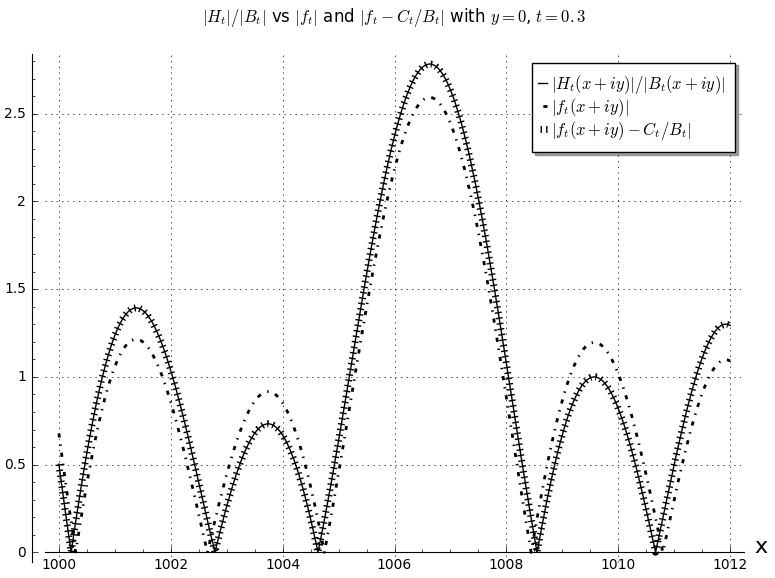
\includegraphics[width=0.6\linewidth]{Extra_RS_term.png}
  \caption{Comparison of $|f_t(x+iy)|$, $|f_t(x+iy)-\frac{C_t(x+iy)}{B_t(x+iy)}|$ and $|H_t(x+iy)|/|B_t(x+iy)|$ for $y=0$, $t=0.3$, $1000 \leq x \leq 1012$.}
	\label{htft-c}
\end{figure}

In addition to establishing upper bounds such as Theorem \ref{new-upper}, one can use Theorem \ref{eff} and Corollary \ref{zero-test} (together with variants in slightly larger regions than \eqref{region}, for instance if $y$ is allowed to be as large as $10$) to obtain asymptotic control on the zeroes of $H_t$, refining previous work of Ki, Kim, and Lee \cite{kkl}.  Indeed, in Section \ref{asymptotic-sec} we will establish

\begin{theorem}[Distribution of zeroes of $H_t$]\label{Zero}  Let $0 < t \leq 1/2$, let $C>0$ be a sufficiently large absolute constant, and let $c>0$ be a sufficiently small absolute constant.  For $x \geq 4\pi$, define
$$ g(x,t) \coloneqq  \frac{x}{4\pi} \log \frac{x}{4\pi} - \frac{x}{4\pi} + \frac{11}{8} + \frac{t}{16} \log \frac{x}{4\pi} $$
and all $n \geq C$, let $x_n$ be the unique real number greater than $4\pi$ such that
\begin{equation}\label{lip}
 g(x_n,t) = n.
\end{equation}
(This is well-defined since the $g(x,t)$ is increasing in $x$ for $x \geq 4\pi$.)
\begin{itemize}
\item[(i)]  If $x \geq \exp(\frac{C}{t})$ and $H_t(x+iy)=0$, then $y=0$, and
$$ x = x_n + O(x^{-ct})$$
for some $n$.  
\item[(ii)]  Conversely, for each $n \geq \exp( \frac{C}{t} )$ there is exactly one zero $H_t$ in the disk $\{ x+iy: |x+iy - x_n| \leq \frac{c}{\log x_n} \}$ (and by part (i), this zero will be real and lie within $O(x^{-ct})$ of $x_n$).
\item[(iii)]  If $X \geq \exp(\frac{C}{t})$, the number $N_t(X)$ of zeroes with real part between $0$ and $X$ (counting multiplicity) is
$$ N_t(X) = g(X,t) + O(1).$$
\item[(iv)]  For any $X \geq 0$, one has
$$ N_t(X+1) - N_t(X) \leq O( \log(2+X) )$$
and
$$ N_t(X) = g(X,t) + O( \log(2+X) ).$$
\end{itemize}
Here and in the sequel we use $X = O(Y)$ to denote the estimate $|X| \leq AY$ for some constant $A$ that is absolute (in particular, $A$ is independent of $t$ and $C$).
\end{theorem}

Roughly speaking, these estimates tell us that the zeroes of $H_t$ behave (on macroscopic scales) like those of $H_0$ in the region $x = O(\exp(O(1/t)))$, and are very evenly spaced (and on the real axis) outside of this range.  The factor $\frac{t}{16} \log \frac{x_n}{4\pi}$ in \eqref{lip} indicates that as time $t$ advances, the zeroes (or at least those with large values of $x$) will tend to move towards the origin at a speed of approximately $\frac{\pi}{4}$.  Although we will not prove this here, the conclusions (i) and (iii) suggest that one in fact has an asymptotic of the form
$$ N_t(X) = \left\lfloor g(X,t) + O( X^{-ct} ) \right\rfloor$$
when $X \geq \exp(C/t)$; in particular (since the sawtooth function $x - \lfloor x \rfloor$ has average value $\frac{1}{2}$) one would have the heuristic approximation
$$ N_t(X) \approx \frac{X}{4\pi} \log \frac{X}{4\pi} - \frac{X}{4\pi} + \frac{7}{8} + \frac{t}{16} \log \frac{X}{4\pi} $$
 after performing some averaging in $X$, thus recovering the familiar $\frac{7}{8}$ term in the usual averaged asymptotics for $N_0(X)$.

\begin{figure}[ht!]
  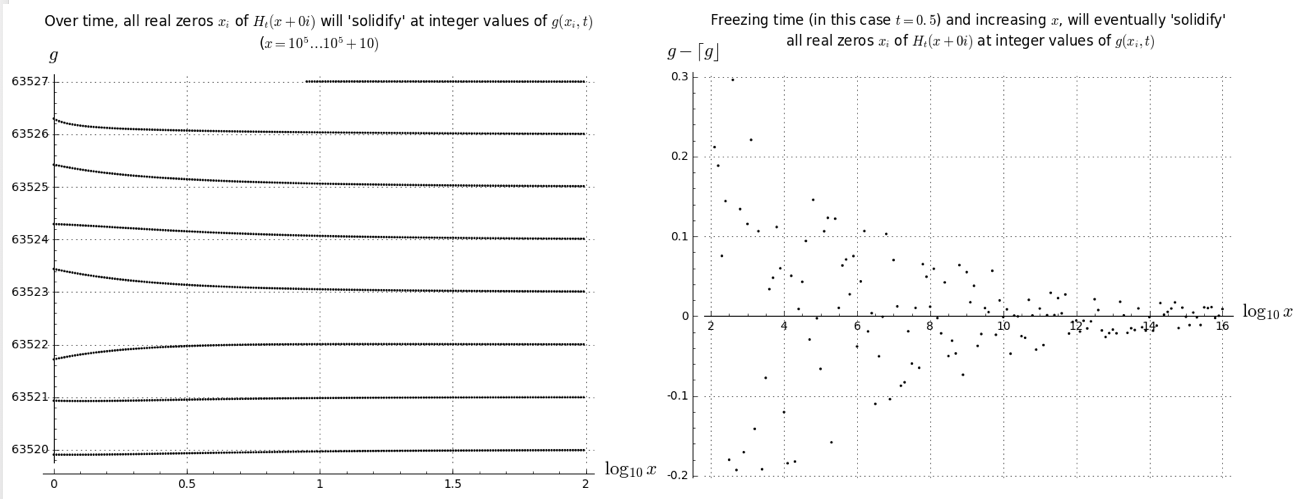
\includegraphics[width=1.0\linewidth]{Integerconvergence_t_and_x_direction.png}
  \caption{The real zeroes $x_i$ of $H_t$ will converge to integer values of $g(x_i,t)$ when $t$ (left) and/or $x$ (right) increases.}
\label{integer_conv_zeros}
\end{figure}

The results in Theorem \ref{Zero} refine previous results of Ki, Kim, and Lee \cite[Theorems 1.3, 1.4]{kkl}, which gave similar results but with constants that depended on $t$ in a non-uniform (and ineffective) fashion, and error terms that were of shape $o(1)$ rather than $O(x^{-ct})$ in the limit $x \to \infty$ (holding $t$ fixed).  The results may also be compared with those in \cite{arias-lune}, who (in our notation) show that assuming RH, the zeroes of $H_0$ are precisely the solutions $x_n$ to the equation
$$ \frac{1}{2\pi} \mathrm{arg}\left( - e^{2 i \vartheta(x_n/2)} \frac{\zeta'(\frac{1-ix_n}{2})}{\zeta'(\frac{1+ix_n}{2})}\right) = n $$
for integer $n$, where $-\vartheta(t)$ is the phase of $\zeta(\frac{1}{2}+it)$ and one chooses a branch of the argument so that the left-hand side is $-\frac{1}{2}$ when $x_n=0$.

\begin{remark}  One can draw an analogy between the various potential behaviours of zeroes of $H_t$ and the three classical states of matter.  A ``gaseous'' state corresponds to the situation in which some fraction of the zeroes of $H_t$ are strictly complex.  A ``liquid'' state corresponds to a situation in which the zeroes are real, but disordered (with highly unequal spacings between zeroes).  A ``solid'' state corresponds to a situation in which the zeroes are real and arranged roughly in an arithmetic progression.  Thus for instance the Riemann hypothesis and the GUE hypothesis assert (roughly speaking) that the zeroes of $H_0$ should exhibit liquid behaviour everywhere, while Theorem \ref{Zero} asserts that the zeroes of $H_t$, $t>0$ ``solidify'' in the region $x \geq \exp(C/t)$.  Below this region we expect liquid behaviour.  In general, as the parameter $t$ increases, the zeroes appear\footnote{This is the picture for positive $t$ at least.  As $t$ becomes very negative, it appears that the ``gaseous'' zeroes become more ordered again, for instance organizing themselves into curves in the complex plane.  See \cite{sharkfin} for further discussion of this phenomenon.} to ``cool'' down, transitioning from gaseous to liquid to solid type states; see \cite{brad} for some formalisations of this intuition. 
\end{remark}

\subsection{About this project}

This paper is part of the \emph{Polymath project}, which was launched
by Timothy Gowers in February 2009 as an experiment to see if research
mathematics could be conducted by a massive online collaboration.
The current project (which was administered by Terence Tao) is the fifteenth
project in this series.  Further information on the Polymath project can be
found on the web site {\tt michaelnielsen.org/polymath1}.  Information
about this specific project may be found at
\begin{center}
\small{{\tt michaelnielsen.org/polymath1/index.php?title=De\_Bruijn-Newman\_constant}}
\end{center}
and a full list of participants and their grant acknowledgments may be
found at
\begin{center}
\small{{\tt michaelnielsen.org/polymath1/index.php?title=Polymath15\_grant\_acknowledgments}}
\end{center}

\section{Notation}

We use the standard branch $\Log$ of the logarithm to define the standard complex powers $z^w \coloneqq \exp( w \Log z)$, and in particular define the standard square root $\sqrt{z} \coloneqq z^{1/2} = \exp( \frac{1}{2} \Log z)$.  We record the familiar gaussian identity
\begin{equation}\label{gaussian}
 \int_\R \exp\left(-(au^2+bu+c)\right)\ du = \sqrt{\frac{\pi}{a}} \exp\left( \frac{b^2}{4a} - c\right)
\end{equation}
for any complex numbers $a,b,c$ with $\mathrm{Re} a > 0$.

When using order of magnitude notation such as $O_{\leq}(X)$, any expression of the form $A=B$ using this notation should be interpreted as the assertion that any quantity of the form $A$ is also of the form $B$, thus for instance $O_{\leq}(1) + O_{\leq}(1) = O_{\leq}(3)$.  (In particular, the equality relation is no longer symmetric with this notation.)

If $F$ is a meromorphic function, we use $F'$ to denote its derivative.  We also use $F^*$ to denote the reflection $F^*(s) := \overline{F(\overline{s})}$ of $F$.  Observe from analytic continuation that if $F:\Omega \to \C$ is holomorphic on a connected open domain $\Omega \subset \C$ containing an interval in $\R$, and is real-valued on $\Omega \cap \R$, then it is equal to its own reflection: $F = F^*$ (since the holomorphic function $F - F^*$ has an uncountable number of zeroes).

%We use $x_+ \coloneqq \max(x,0)$ to denote the positive part of a real number $x$.  
%If $E$ is a statement, we use $1_E$ to denote its indicator, thus $1_E=1$ when $E$ is true and $1_E=0$ when $E$ is false.  For natural numbers $d,n$, we use $d|n$ to denote the assertion that $d$ divides $n$.